\chapter{Results}
\label{ch:results}
In this chapter achieved results are presented. I tested each method on four datasets as described in chapter \ref{ch:sw} and \ref{ch:testing}. Next I will shortly described possible setups of each of the three methods I used in the experiments. It will be  followed by discussion of the results of test divided into sections by the four datasets.
I have divided the experiments by the four datasets and made comparisons. Prediction methods were examined with a different setting of parameters where possible.


\subsection*{EasyOCR}
I used the version 1.5.0 of the EasyOCR python package. The experiments were run using a GPU. I used two different settings for EasyOCR engine -- the basic one which tends to detect and recognize text as single word objects and the second setting merges close words together creating text lines of words that belong together.

\subsection*{Keras-OCR}
The keras\_ocr-0.9.1 package for Python was used in experiments. It was necessary to compute the predictions on GPU, due to the limited GPU on Google Colab and the size of the images needed to be processed one by one although Keras allows to process images in batches. Keras-OCR predictions are case insensitive, because the default model does not support uppercase letters. I trained the Keras recognition model on SCUT-CTW1500 dataset (on the one thousand training images), first a trained the default model with lower case alphabet, then with the same alphabet and a space character and finally with uppercase letters and a set of special characters. In the results discussion it will be shown that after training the model does not offer better results than the original model. THe original model is already very successful and was well trained on much larger datasets.

Each of the training took about an hour on Google Colab GPU. I set 100 epochs and an early stopping based on the value of validation loss. The validation data were taken from the train data as 20\% of the whole training part. First the I used early stopping after 10 non decreasing values, then after 30, but in both cases the model could not get any better than 14\% validation loss.

% graph

\subsection*{Tesseract}
The version of Tesseract installed on Google Colab is tesseract 4.0.0-beta.1 with leptonica-1.75.3, which means that the LSTM network is available. For testing I used the OCR Engine mode (OEM) 3, that is Legacy + LSTM engines. As for Page segmentation modes (PSM) I used numbers 3, 4, 6, 8 and 11, which are "Fully automatic page segmentation, but no OSD. (Default)", "Assume a single column of text of variable sizes.",  "Assume a single uniform block of text.",  "Treat the image as a single word." and "Sparse text. Find as much text as possible in no particular order." respectively. I used PSM 3 only initially and dropped it beacuse prediction was strongly inefficient, so it is not included in result statistics. PSM 8 was used for testing Tesseract with CRAFT, because CRAFT crops an image into segments where there is only one word (or a short text line), therefore Tesseract needed to treat the image as a single word. The rest of mentioned PSMs were applied for examining the behavior of pure Tesseract engine. 




\subsection*{Born-Digital}

First, the Born-Digital Images dataset was tested with images in predictions and ground truth were set to be in lowercase and all special characters except for space were removed. There were 13 different testing runs with three tested methods.  In Figure \ref*{Im:resBD} are the results of this testing and in Table \ref*{Tab:resBD} is corresponding information about each run. 

The best CER value was achieved by tuned EasyOCR engine, where no split was done on predicted text (letter D in Fig. \ref*{Im:resBD}). We can see from the graph and table, that EasyOCR and keras-OCR had significantly better results than Tesseract. Also it can be said that tuning of EasyOCR model results in higher both IoU and CER of approximately 20\% more than with basic EasyOCR setup of parameters. Keras-OCR performs similarly with split and no split option and in both cases gives satisfactory results. The best IoU score was equal to $64.6\%$ (letters G and H) and belongs to Keras-OCR model. Tuned EasyOCR can get up to $60.3\%$ without tuning $20\%$ lower than that.

When we compare Tesseract with its own detection model and Tesseract with CRAFT tool, we can see that CRAFT increases the CER metric by more than 12\%, however the IoU metric fluctuates for all cases around 50\%. Whether the image is in RGB color scheme or in grayscale has only a little impact on the results, generally it differed only by about 2\%. Same minor difference is when split or no split option is set. If the Otsu thresholding was performed and the image was then binarized, results were worse than when Tesseract itself performs the binarization. Better results were when PSM tesseract parameter was set to 11 rather then PSM 4.

{
\begin{figure}[hbtp!]
    \centering
    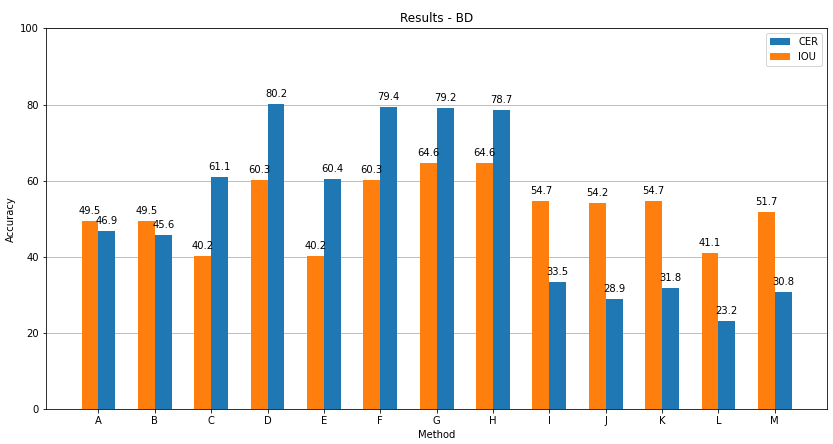
\includegraphics[width=\textwidth]{obrazky/grafy/resBD.png}
    \caption{Results of experiments performed on Born-Digital Images dataset. Information about each method is in Table \ref*{Tab:resBD}.}
    \label{Im:resBD}
\end{figure}
\begin{table}[!hbt]
    \centering
    \begin{tabular}{|l|l|l|}
    \hline
        Key & Method & Properties \\ \hline
        A & tesseract+CRAFT &  no split, psm8\\ 
        B & tesseract+CRAFT &  split, psm8\\ \hline
        C & easyOCR &  no split, no tuning\\ 
        D & easyOCR &  no split, tuning\\ 
        E & easyOCR &  split, no tuning\\ 
        F & easyOCR &  split, tuning\\ \hline
        G & keras-OCR &  no split\\ 
        H & keras-OCR &  split\\ \hline
        I & tesseract & colored, no split, psm11\\ 
        J & tesseract & binary, split, psm11\\ 
        K & tesseract & colored, split, psm11\\ 
        L & tesseract & binary, split, psm4\\ 
        M & tesseract & colored, split, psm4\\ \hline
    \end{tabular}
    \caption{A table of keys for methods and parameters of experiments performed on Born-Digital Images dataset for Figure \ref*{Im:resBD}.}
    \label{Tab:resBD}
\end{table}
}

Next I performed tests with case sensitive option and with special characters included.

\subsection*{SCUT-CTW1500 dataset}
The SCUT-CTW1500 dataset was again first tested with predictions and ground truth were set to be in lowercase and all special characters except for space were removed. 14 different testing were run.  In Figure \ref*{Im:resCTW} are the results of the testing and the corresponding information about each run is in Table \ref*{Tab:resCTW}. 

This time the best CER value ($76.4\%$) was achieved by keras-OCR model, where split was performed on predicted text (letter H in Fig. \ref*{Im:resCTW}). It can be seen from the graph and table, that EasyOCR and keras-OCR had again significantly better results than Tesseract. In testing of CTW1500 dataset this time keras-OCR generally performed better than EasyOCR in CER metric by roughly 10\%. The tuning of EasyOCR model results in lower both IoU and CER of approximately 2\% less than with basic EasyOCR setup of parameters. This might by probably due to the fact that EasyOCR model was trained on data similar to CTW1500 dataset rather then Born-Digital Images dataset Keras-OCR performs simlarly with split and no split option and in both cases gives satisfactory results.

The Comparison of Tesseract with its own detection model and Tesseract with CRAFT tool shows that with CRAFT the CER metric increased by almost than 20\% as well as the IoU metric that increased by more than 30\%. Plain Tesseract results are again the worst and are not heavily influenced by color scheme or slight scaling changes. 

\begin{figure}[hbtp!]
    \centering
    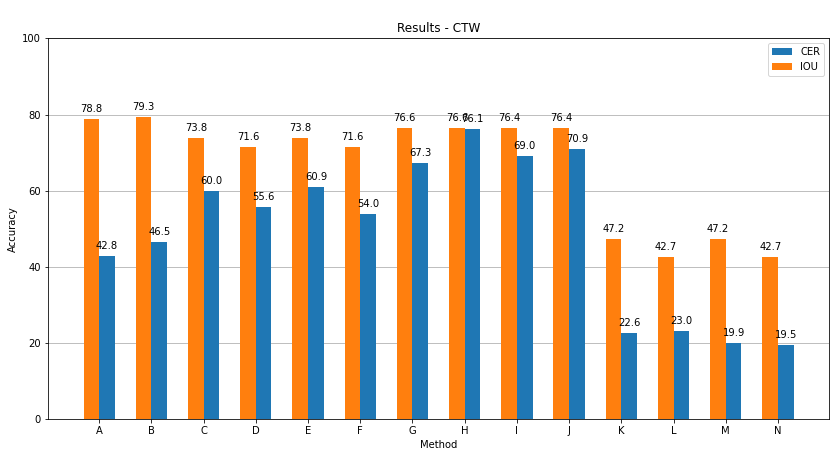
\includegraphics[width=\textwidth]{obrazky/grafy/resCTW.png}
    \caption{Results of experiments performed on CTW dataset. Information about each method is in Table \ref*{Tab:resCTW}.}
    \label{Im:resCTW}
\end{figure}
\begin{table}[!ht]
    \centering
    \begin{tabular}{|l|l|l|}
    \hline
        Key & Method & Properties \\ \hline
        A & tesseract+CRAFT & no split \\ 
        B & tesseract+CRAFT & split \\ \hline
        C & easyOCR & nosplit, notuning \\ 
        D & easyOCR & no split, tuning \\ 
        E & easyOCR & split, notuning \\ 
        F & easyOCR & split, tuning \\ \hline
        G & keras-OCR & original image width, no split \\ 
        H & keras-OCR & original image width, split \\ 
        I & keras-OCR & original image width, split, trained spaces \\ 
        J & keras-OCR & original image width, split, trained \\ \hline
        K & tesseract & 3000px image width, no split \\ 
        L & tesseract & color, no split, psm11 \\ 
        M & tesseract & split, psm11\\ 
        N & tesseract & color, split, psm11 \\ \hline
    \end{tabular}
    \caption{A table of keys for methods and parameters of experiments performed on SCUT-CTW1500 dataset for Figure \ref*{Im:resCTW}.}
    \label{Tab:resCTW}
\end{table}

\subsection*{KAIST Scene Text Database}

Testing of performance of the three methods on KAIST dataset with case insensitivity and no special characters was done in 22 different runs. Eight of them were on KAIST bitmap images, as these images do not have a misleading background the results are significantly better than on original photographes. The results can be seen in Figure \ref*{Im:resK} and the corresponding information is in Table \ref*{Tab:resK}. 
The best results on the bitmap images part of KAIST dataset were performed by EasyOCR dataset with no splitting and CER value is $82.2\%$ high (letter B in Fig. \ref*{Im:resK}). This method with the same setup is also best with KAIST dataset unedited photographs. Due to the character of the dataset for all cases the no split option is distinctly better. 

Keras-OCR had slightly lower values of CER than EasyOCR and IoU values are even lower by generally 15\%. Still it is by 20\% higher than results of plain Tesseract and comparable with Tesseract and CRAFT combination. Tesseract had this time best but still way too low results with PSM 6. PSM 4 led to CER value as low as 18\%. Color scheme did not have a distinguishable impact on the results.
 
\begin{figure}[hbtp!]
    \centering
    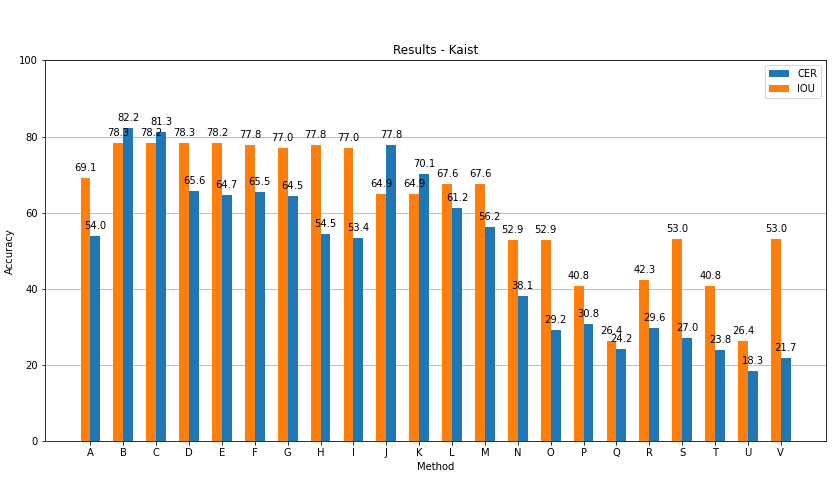
\includegraphics[width=\textwidth]{obrazky/grafy/resKaist.png}
    \caption{Results of experiments performed on KAIST Scene Text Database. Information about each method is in Table \ref*{Tab:resK}.}
    \label{Im:resK}
\end{figure}
\begin{table}[!ht]
    \centering
    \begin{tabular}{|l|l|l|}
    \hline
        Key & Method & Properties \\ \hline
        A & tesseract+CRAFT & no split \\ \hline
        B & easyOCR & bmp, no split, no tuning \\ 
        C & easyOCR & bmp, no split, tuning \\ 
        D & easyOCR & bmp, split, no tuning \\ 
        E & easyOCR & bmp, split, tuning \\ 
        F & easyOCR & no split, no tuning \\ 
        G & easyOCR & no split, tuning \\ 
        H & easyOCR & split, no tuning \\ 
        I & easyOCR & split, tuning \\ \hline
        J & keras-OCR & bmp, no split \\ 
        K & keras-OCR & bmp, split \\ 
        L & keras-OCR & no split \\ 
        M & keras-OCR & split \\ \hline
        N & tesseract & bmp, no split, psm11 \\ 
        O & tesseract & bmp, split, psm11 \\ 
        P & tesseract & colored, no split, psm11 \\ 
        Q & tesseract & colored, no split, psm4 \\ 
        R & tesseract & colored, no split, psm6 \\ 
        S & tesseract & no split, psm11 \\ 
        T & tesseract & colored, split, psm11 \\ 
        U & tesseract & colored, split, psm4 \\ 
        V & tesseract & split, psm11 \\ \hline
    \end{tabular}
    \caption{A table of keys for methods and parameters of experiments performed on KAIST Scene Text Database for Figure \ref*{Im:resK}.}
    \label{Tab:resK}
\end{table}



% Training took one hour and stopped after 57 epochs ,10.979148864746094,20.5778751373291. Continued training.

% trained no spaces 
% [[('bruno', 'brung', 0.2)],
%  [('optique', 'ortinu', 0.42857142857142855),
%   ('optique', 't', 0.8571428571428571)],
%  [('promotion', 'mgtioa', 0.5555555555555556),
%   ('promotion', 'rro', 0.7777777777777778)],
%  [('la', 'bne', 1.0),              ('paire', 'paite', 0.2)]]
%  [[('panns', 'aine', 0.6)],
%  [('1958', '1953', 0.25), ('since', 'simce', 0.2)],
%  [('food', 'food', 0.0), ('real', 'rea', 0.25)]]
%   ('la', 'loz', 0.6666666666666666),
%                 ('paire', 'paite', 0.2)]]
%                 [[('panns', 'aine', 0.6)],
%                 [('1958', '1953', 0.25), ('since', 'simce', 0.2)],
%                 [('food', 'food', 0.0), ('real', 'rea', 0.25)]]


% CTW
% training with special chars case insensitive no special split
% [[('bruno', 'bruns', 0.2)],
%  [('optique', 'optoue', 0.2857142857142857), ('optique', 'srss', 1.0)],
%  [('promotion', 'bre', 0.8888888888888888),
%   ('promotion', 'motion', 0.3333333333333333)],
%  [('2eme', 'enne', 0.75), ('la', 'le', 0.5), ('la', 'salls', 0.8)]]

%  s no splitem 60 to je fakt malo ani ne v grafu

%  velka pismena a znaky
%  [[('BRUNO', 'BRUNS', 0.2)],
%  [('OPTIQUE', 'OPTOUE', 0.2857142857142857), ('OPTIQUE', 'SRSS', 1.0)],
%  [('PROMOTION', 'BRE', 0.8888888888888888),
%   ('PROMOTION', 'MOTION', 0.3333333333333333)],
%  [('2eme', 'enne', 0.75), ('La', 'Le', 0.5), ('La', 'Salls', 0.8)]]

%  [[('DOUGLASTON', 'BOUGLASTON', 0.1)],
%  [('E-313', 'E313', 0.2)],
%  [('L164', 'Lbl6w', 0.6)],
%  [('F.D.N.Y.', 'EDNY', 0.625)]]

% BD

% nula

% [[('flying', 'tying', 0.3333333333333333)],
%  [('today', 'todoy', 0.2)],
%  [('means', 'eons', 0.4)],
%  [('vueling', 'VUelnng', 0.42857142857142855)],
%  [('GET', 'GET', 0.0)],
%  [('', 'AVAY.', 1)],
%  [('1.000.000', '1.000.000', 0.0)],
%  [('SEATS', 'SEATS', 0.0)],
%  [('FROM', 'FRON', 0.25)],
%  [('30€', '303', 0.3333333333333333)],
%  [('Book', 'BOOK', 0.75)],
%  [('now!', 'nowi', 0.25)]]

% Case sensitivity


% when default model is used and special characters and case sensitivity of ground truth labels is observed CER accuracy reaches only less than thirty percent. 


\subsection*{Vienna City Poster Dataset}

The Vienna City Poster Dataset was detected and recognized with the same method as previously mentioned datasets. Even though the dataset has only a little over 250 images, it is that large that the RAM size available in Google Colab struggled to work with the dataset as whole I had to split the dataset into two parts and perform computations on them separately. Then I combined the corresponding results. Specifically, the first group included first 123 images, the second the rest, where data were sorted by name of the files.

I used different parameters that can be set in each method. However, in the result table \ref*{Tab:resV} and graph \ref*{Im:resV} I selected only the best ones within each method. Thus the results contains     thirteen CER and IoU values. In the featured results for all cases except one I tested only alphanumeric characters without the sensitivity to their case.

Due to the fact that this dataset is mainly in German language, in all models I set German as the language that is to be predicted. The defualt was English for all models. I implemented possible language correction which takes common syllables that appear in German. The function is described in \ref{sec:other}. For some predictors these corrections were not necessary and predicted similarly without them. 

\begin{figure}[hbtp!]
    \centering
    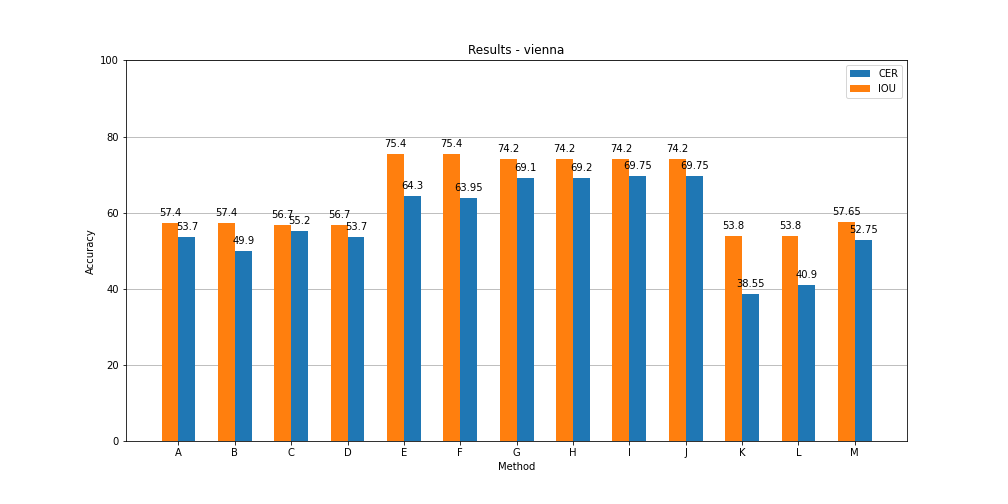
\includegraphics[width=\textwidth]{obrazky/grafy/resvienna.png}
    \caption{Results of experiments performed on Vienna City Poster Dataset. Information about each method is in Table \ref*{Tab:resV}.}
    \label{Im:resV}
\end{figure}

\begin{table}[!ht]
    \centering
    \begin{tabular}{|l|l|l|}
    \hline
        Key & Method & Properties \\ \hline
        A & Tesseract+CRAFT & split \\
        B & Tesseract+CRAFT & case sensitive, includes special characters, split \\ \hline
        C & easyOCR & no split, no tuning, correction\\
        D & easyOCR & no split, no tuning, no correction \\
        E & easyOCR & no split, tuning, correction\\
        F & easyOCR & split, tuning, correction" \\ \hline
        G & keras-OCR & no split, correction" \\
        H & keras-OCR & no split, no correction" \\ 
        I & keras-OCR & split, correction" \\ 
        J & keras-OCR & split, no correction" \\ \hline
        K & tesseract & no split, psm11" \\ 
        L & tesseract & split, psm11" \\ 
        M & tesseract & split, psm4" \\ \hline
    \end{tabular}
    \label{Tab:resV}
\end{table}

The best results were obtained by EasyOCR and Keras-OCR. The highest IoU score is equal to $75.4\%$ and it belongs to EasyOCR method with its parameters tuned to create tighter bounding boxes than pure EasyOCR (letters E and F in Fig. \ref*{Im:resV}). In this case the CER values ranged around $64\%$ and correction for German language was involved.
Keras-OCR is responsible for the highest CER value -- $69.75\%$, for both with and without correction. Though the IoU value is sligtly smaller than the best one -- $74.2\%$ (letters G-J). 

As EasyOCR is able to predict also special characters and can be sensitive to case in its result I tested the two best settings (letters E and F) with this option. The CER scores lowered by approximately $3.5\%$. Which means that even with case sensitivity and more characters the model can give very good results. In contrast with Keras-OCR which cannot predict special characters and ignores text case without training. To gain this aibility, I trained the Keras-OCR model on the Vienna Dataset. I used the the second group of the dataset data as a training images and the first 123 images as testing ones. After seventeen minutes, which accords with twenty epochs, the training ended, because last ten epochs the validation loss stopped decreasing. Unfortunately the trainind dataset would need more data. After tests the IoU score was equal to $73.2\%$ and CER score was $72.1\%$ without my language corrections and with split applied to predictions. These numbers shows that Keras-OCR outperforms other models in both with simple characters and with special characters.

Tesseract (letters K-M in Fig. \ref*{Im:resV}) performance, similarly as with other tested datasets, was the worst. Usually the problem was caused by poor detection of the individual words. Very often objects were detected as letters, this happens when the PSM 11 was used. This eleventh option --  find as much text as possible in no particular order -- sounds ideal, because in the posters the text mainly does not keep an order and is present in various locations, orientations and sizes. CER values ranged around $40\%$. However, PSM 4, which assumes a single column of text of variable sizes, performed better with alike accuracy as Tesseract recognizer with CRAFT detector or as untuned EasyOCR, CER values reached neraly up to $53\%$. This comparision was unrealistic for scene text datasets.

When CRAFT package was used as a detector and cropped detected words were sent to Tesseract recognizing tool and treated as a single word (PSM 8). Then the CER score was equal to $53.7\%$ (letters A and B in Fig. \ref*{Im:resV}).


% ---------------------------- Result Conclusion --------------------------------------
\section*{Result Conclusion}

The previous section contains a discussion over achieved results. From this discussion it can be concluded that Keras-OCR and EasyOCR have the best results for all datasets. The CER score fluctuates between $65\%$ and $80\%$. The upper boundary is very good and the lower also indicates acceptable predictions. The detection statistics, IoU, for these two winning methods is between $63\%$ and $75\%$.

It can also be concluded that Tesseract gave overall the worst results. When performed on scene text image data, it returned CER value usually around $20\%$, on born-digital data results were around $30\%$ and for the most important Vienna dataset it returned values ranging from $38\%$ to nearly $53\%$. However these numbers are still lower than of any other method. When I changed the default detector in Tesseract to CRAFT detection tool, for all datasets the IoU statistics slightly increased and for the CER statistics a significant rise occured. In cases of SCUT-CTW1500 dataset and KAIST Scene Text Database the CER value doubled. A statement can be made regarding the page segmentation mode 11 of Tesseract tool -- PSM 11, used for images where we want to find as much text as possible, causes that Tesseract finds  much more words in the image and mistakes patterns for letters. This causes that a problem when interpreting the metrics. The IoU can falsely increase, because small false bounding boxes can cover parts of ground truth boxes bounding some large unrecognized word.

In \ref*{ch:appendix} there are examples of images selected from the Vienna City Poster Dataset. Predictions of methods and ground truths are displayed on the images can be compared with each other. I also selected in the examples a couple of images with fonts difficult to recognize.

It is important to say that if there was a bigger labeled dataset for testing the methods, the score values would be more precise and the very difficult fonts and images would not have such an impact on the statistics as they did.